%%
%  ******************************************************************************
%  * #file    Szablon_raportu_EN_Latex.tex
%  * #author  Adrian Wójcik   adrian.wojcik(at)put.poznan.pl
%  *          
%  * #commit  Patryk Kościk   koscikpatryk(at)gmail.com
%  *          Modified the template for Projekt przejsciowy purposes          
%  *          
%  * #version 1.0
%  * #date    09-Mar-2022
%  * #brief   PROJPRZEJ
%  *
%  ******************************************************************************
%%  
\documentclass[11pt, a4paper]{article}

\usepackage{SM_template}

% Wypełnijcie te dyrektywy zgodnie z waszym tematem
% \lab      -> NAZWA CZUJNIKA, np.: 'DHT22'
% \comment  -> Króciutki opis co to, np.: 'Cyfrowy budżetowy czujnik temperatury'
%
\lab{KY-032}
\comment{Wyświetlacz cztero liczbowy siedmiosegmentowy \\ Szymon Kwiatkowski}

% Absolutny zakaz dotykania tego tutaj bo jak dotkiecie to coś jebnie
\university{Politechnika Poznańska}
\faculty{Wydział Automatyki, Robotyki i Elektrotechniki}
\institute{Instytut Robotyki i Inteligencji Maszynowej}
\department{Zakład Sterowania i Elektroniki Przemysłowej}
\addbibresource{bib/7Segment4DigitDisplay.bib}
\nocite{*}


%%
%
% Początek dokumentu
%
%%
\begin{document}

%% Strona tytułowa %%
\mainpage{{7Segment4DigitDisplay/7Segment4DigitDisplay.jpg}}
\newpage

\section*{Opis elementu} \addcontentsline{toc}{section}{Wstęp}
Wyświetlacz 7 segmentowy charakteryzuje się posiadaniem diód które mogą być załączane za pomocą sygnałów, każdy segment zazwyczaj oznacza się jako: A, B, C, D, E, F, G.
\newline
Wyświetlacze takie mogą charakteryzować się posiadaniem wspólnej katody, bądź wspólnej anody. Posiadając wspólną katodę charakteryzuje się posiadaniem jednej linii zasilającej $V_{CC}$, które to zapala diody w zależności od tego w jakim stanie znajduje się stan kolejnych segmentów, natomiast posiadając wspólną anodę posiadamy jedną masę układu i wiele linii zasilających. .Każdy wyświetlacz siedmiosegmentowy posiada następujące przypisanie segmentów:
\begin{figure}[H]
    \centering
    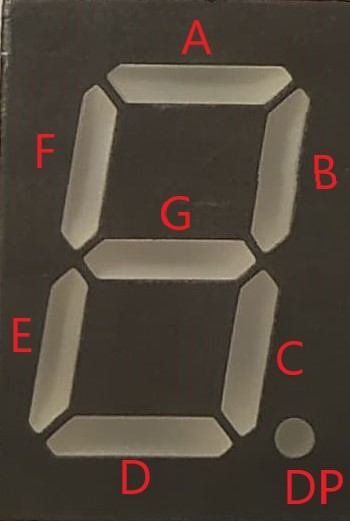
\includegraphics[width=0.3\textwidth]{fig/7Segment4DigitDisplay/zasada_dzialania/1Segment.jpg}
    \caption{Oznaczenia segmentów wyświetlacza}
\end{figure}
Oprócz podstawowych segmentów można również dla wyświetlaczy posiadających więcej niż jedną liczbę wyróżnić pole oznaczone jako DP, co jest skrótem od decimal point, czyli po prostu separatora jedności od części dzięsiętnych. Wyświetlacze które posiadają więcej niż jedną liczbę charakteryzują się z reguły również tym że implementują one pewne uproszczenie które pozwala na zmniejszenie ilości wyprowadzeń wyświetlacza które musimy podłączyć, aby układ poprawnie funkcjonował. Posiadając indywidualne piny dla każdego z wyświetlaczy zakładając że nie posiadałyby one DP łączna ich ilość wyniosłaby $4\times8 = 32$ dla 4 wyświetlaczy siedmiosegmentowych. By zmniejszych tak dużą ilość pinów stostuje się rozwiązanie które polega na tym że wszystkie piny wyświetlacza odpowiadające za zapalnie segmentów są wspólne dla każdej z liczb na nim, natomiast wpisanie wartości na odpowiednią pozycję odbywa się za pomocą wybrania odpowiedniej części wyświetlacza za pomocą osobnych pinów. Oznacza to że w minimalnej postaci będziemy posiadali $7 + 4$, dla wyświetlacza który składa się z 4 wyświetlaczy siedmiosegmentowych. Jak można zauważyć jest to znacząco mniejsza ilość pinów które wykorzystujemy co z kolei pozwala na wykorzystanie układu mikroprocesorowego do wykonywania większej ilości zadań w trakcie jego pracy. Wyświetlacz który będzie rozpatrywany posiada wspólną katodę i 14 pinów co wiąże się z posiadaniem pinu decimal point(1 dodatkowy pin) oraz separatora na środku wyświetlacza(2 dodatkowe piny, jeden to zasilania drugi to masa). Schemat elektryczny takiego moduły wygląda następująco:
\begin{figure}[H]
    \centering
    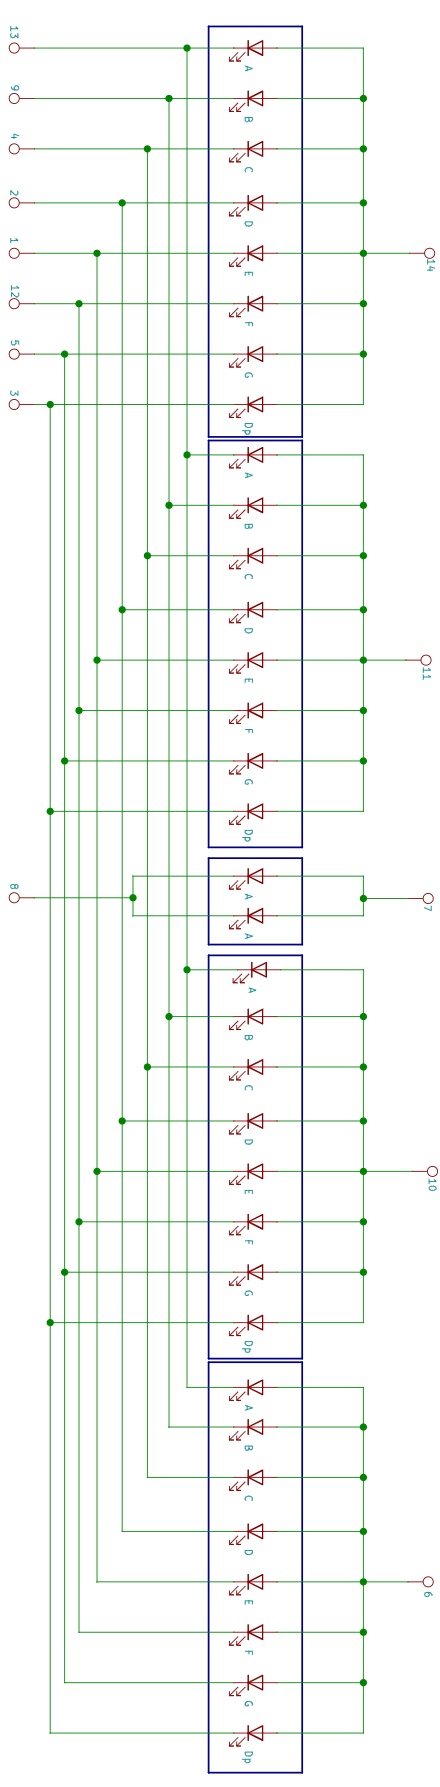
\includegraphics[width=0.3\textwidth]{fig/7Segment4DigitDisplay/polaczenie_modulu/schemat.png}
    \caption{Schemat elektryczny układu}
\end{figure}

Natomiast sama numeracja pinów prezentuje się w poniższy sposób:
\begin{figure}[H]
    \centering
    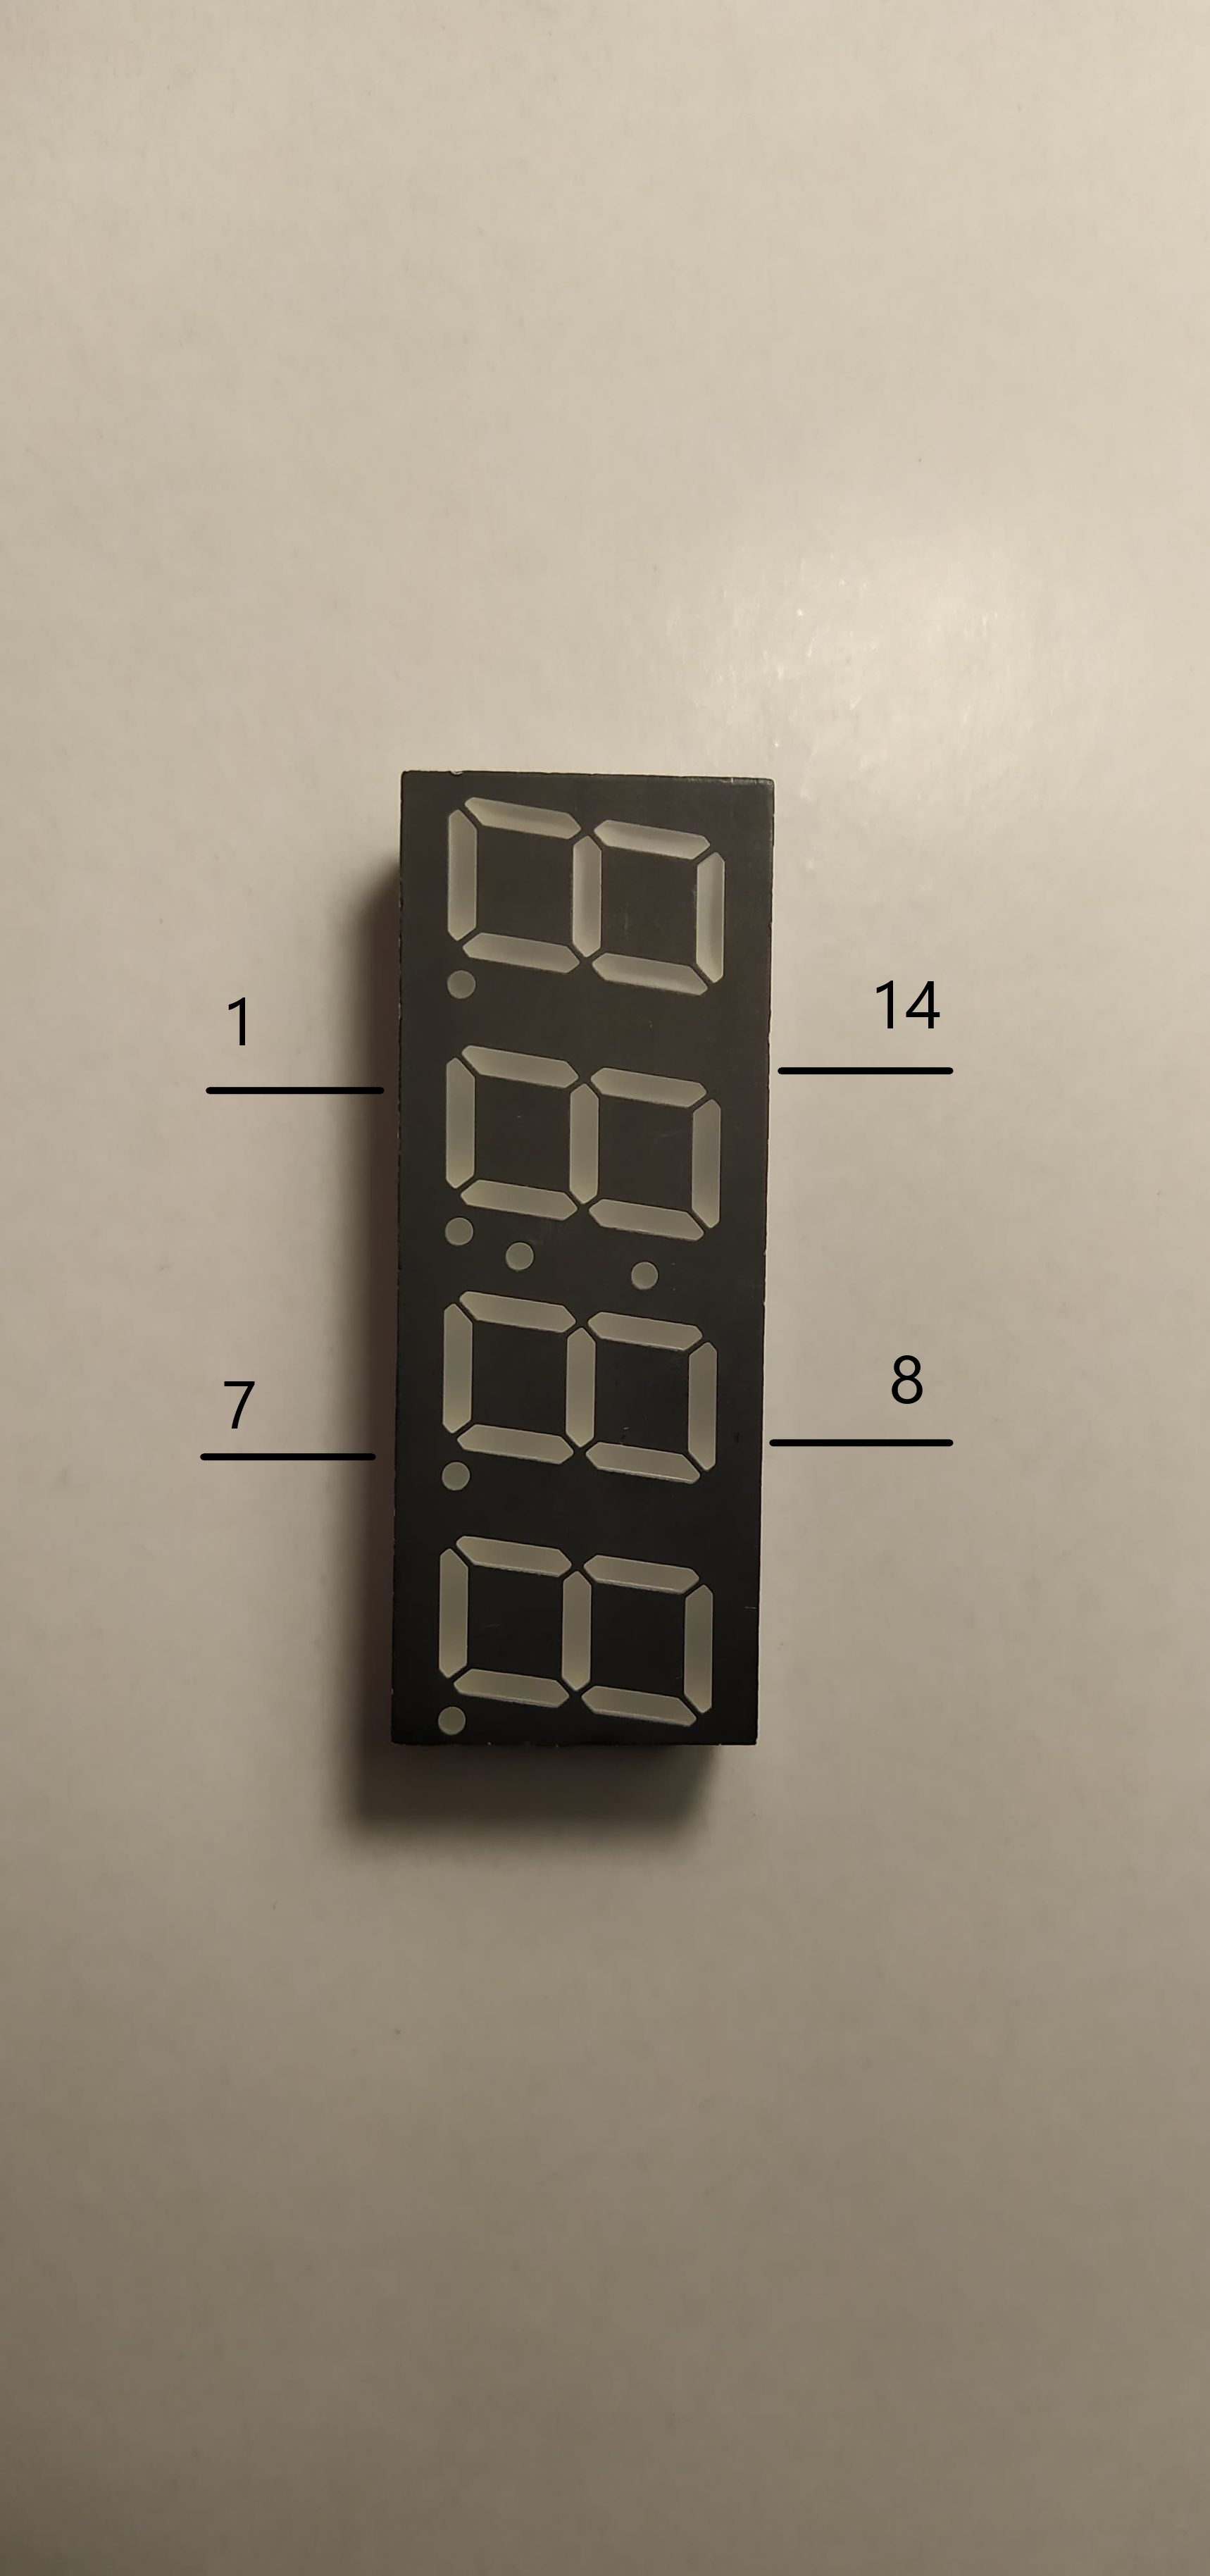
\includegraphics[width=0.3\textwidth]{fig/7Segment4DigitDisplay/polaczenie_modulu/pins.jpg}
    \caption{Numeracja pinów}
\end{figure}



\newpage
\section{Użycie czujnika}
Jak już to było wspomniane wyświetlacze które posiadają wiele liczb charakteryzują się tym że oszczędzają ilość pinów.
Posiadanie mniejszej ilości pinów wiąże się jednak z pewnym wymogiem polegającym na oszukaniu ludzkiego oka podczas pracy wyświetlacza. Polega on na pracy wyświetlacza tak aby wszystkie jego liczby były odświeżane z okresem o wartości maksymalnej 5ms. Jeżeli częstotliwość ta jest mniejsza to liczby będą mniej widoczne, sam wyświetlacz nie wyglądał odpowiednio. Wiąże się to oczywiście z tym że musimy nieustannie zapalać i zagaszać kolejne liczby na wyświetlaczu by każda liczba mogła być osobno wyświetlana, jeżeli tego nie będziemy robić to oczywiście wyświetlane przez nas dane będą nieadekwatne do tego co powinno być wyświetlane. Oznacza to że proces obsługi takiego wyświetlacza wygląda następująco:
\begin{itemize}
    \item Nadanie stanu wysokiego na wejście zasilające danej liczby wyświetlacza
    \item Nadanie stanu niskiego do odpowiednich segmentów zasilania tak aby uzyskać odpowiednie dane wyjściowe na wyświetlaczu dla danej liczby
    \item Wystawienie stanu wysokiego na wszystkie segmenty(Przywrócenie ich do stanu domyślnego)
    \item Przywrócenie stanu niskiego na zasilanie danej liczby wyświetlacza
\end{itemize}
W ten sposób odpowiednio separujemy wyświetlanie na pojedynczych liczbach naszego wyświetlacza, jednocześnie wyświetlając odpowiednie informacje. Oczywiście liczby które wyświetlane muszą zostać odpowiednio zakodowane na segmentach tak aby być w stanie uzyskać odpowiedni efekt końcowy.
\subsection{Implementacja na mikrokontrolerze}
Na płytce ewaluacyjnej NUCLEOF746ZG utworzono program który realizował funkcję sterownika wyświetlacza siedmiosegmentowego. Piny które obrano jako wejścia do wyświetlacza pokrywały się w następujący sposób: D1 = Pin 1, D2 = Pin 2 itd. Wszystkie piny zostały podpięte następująco:
\begin{figure}[H]
    \centering
    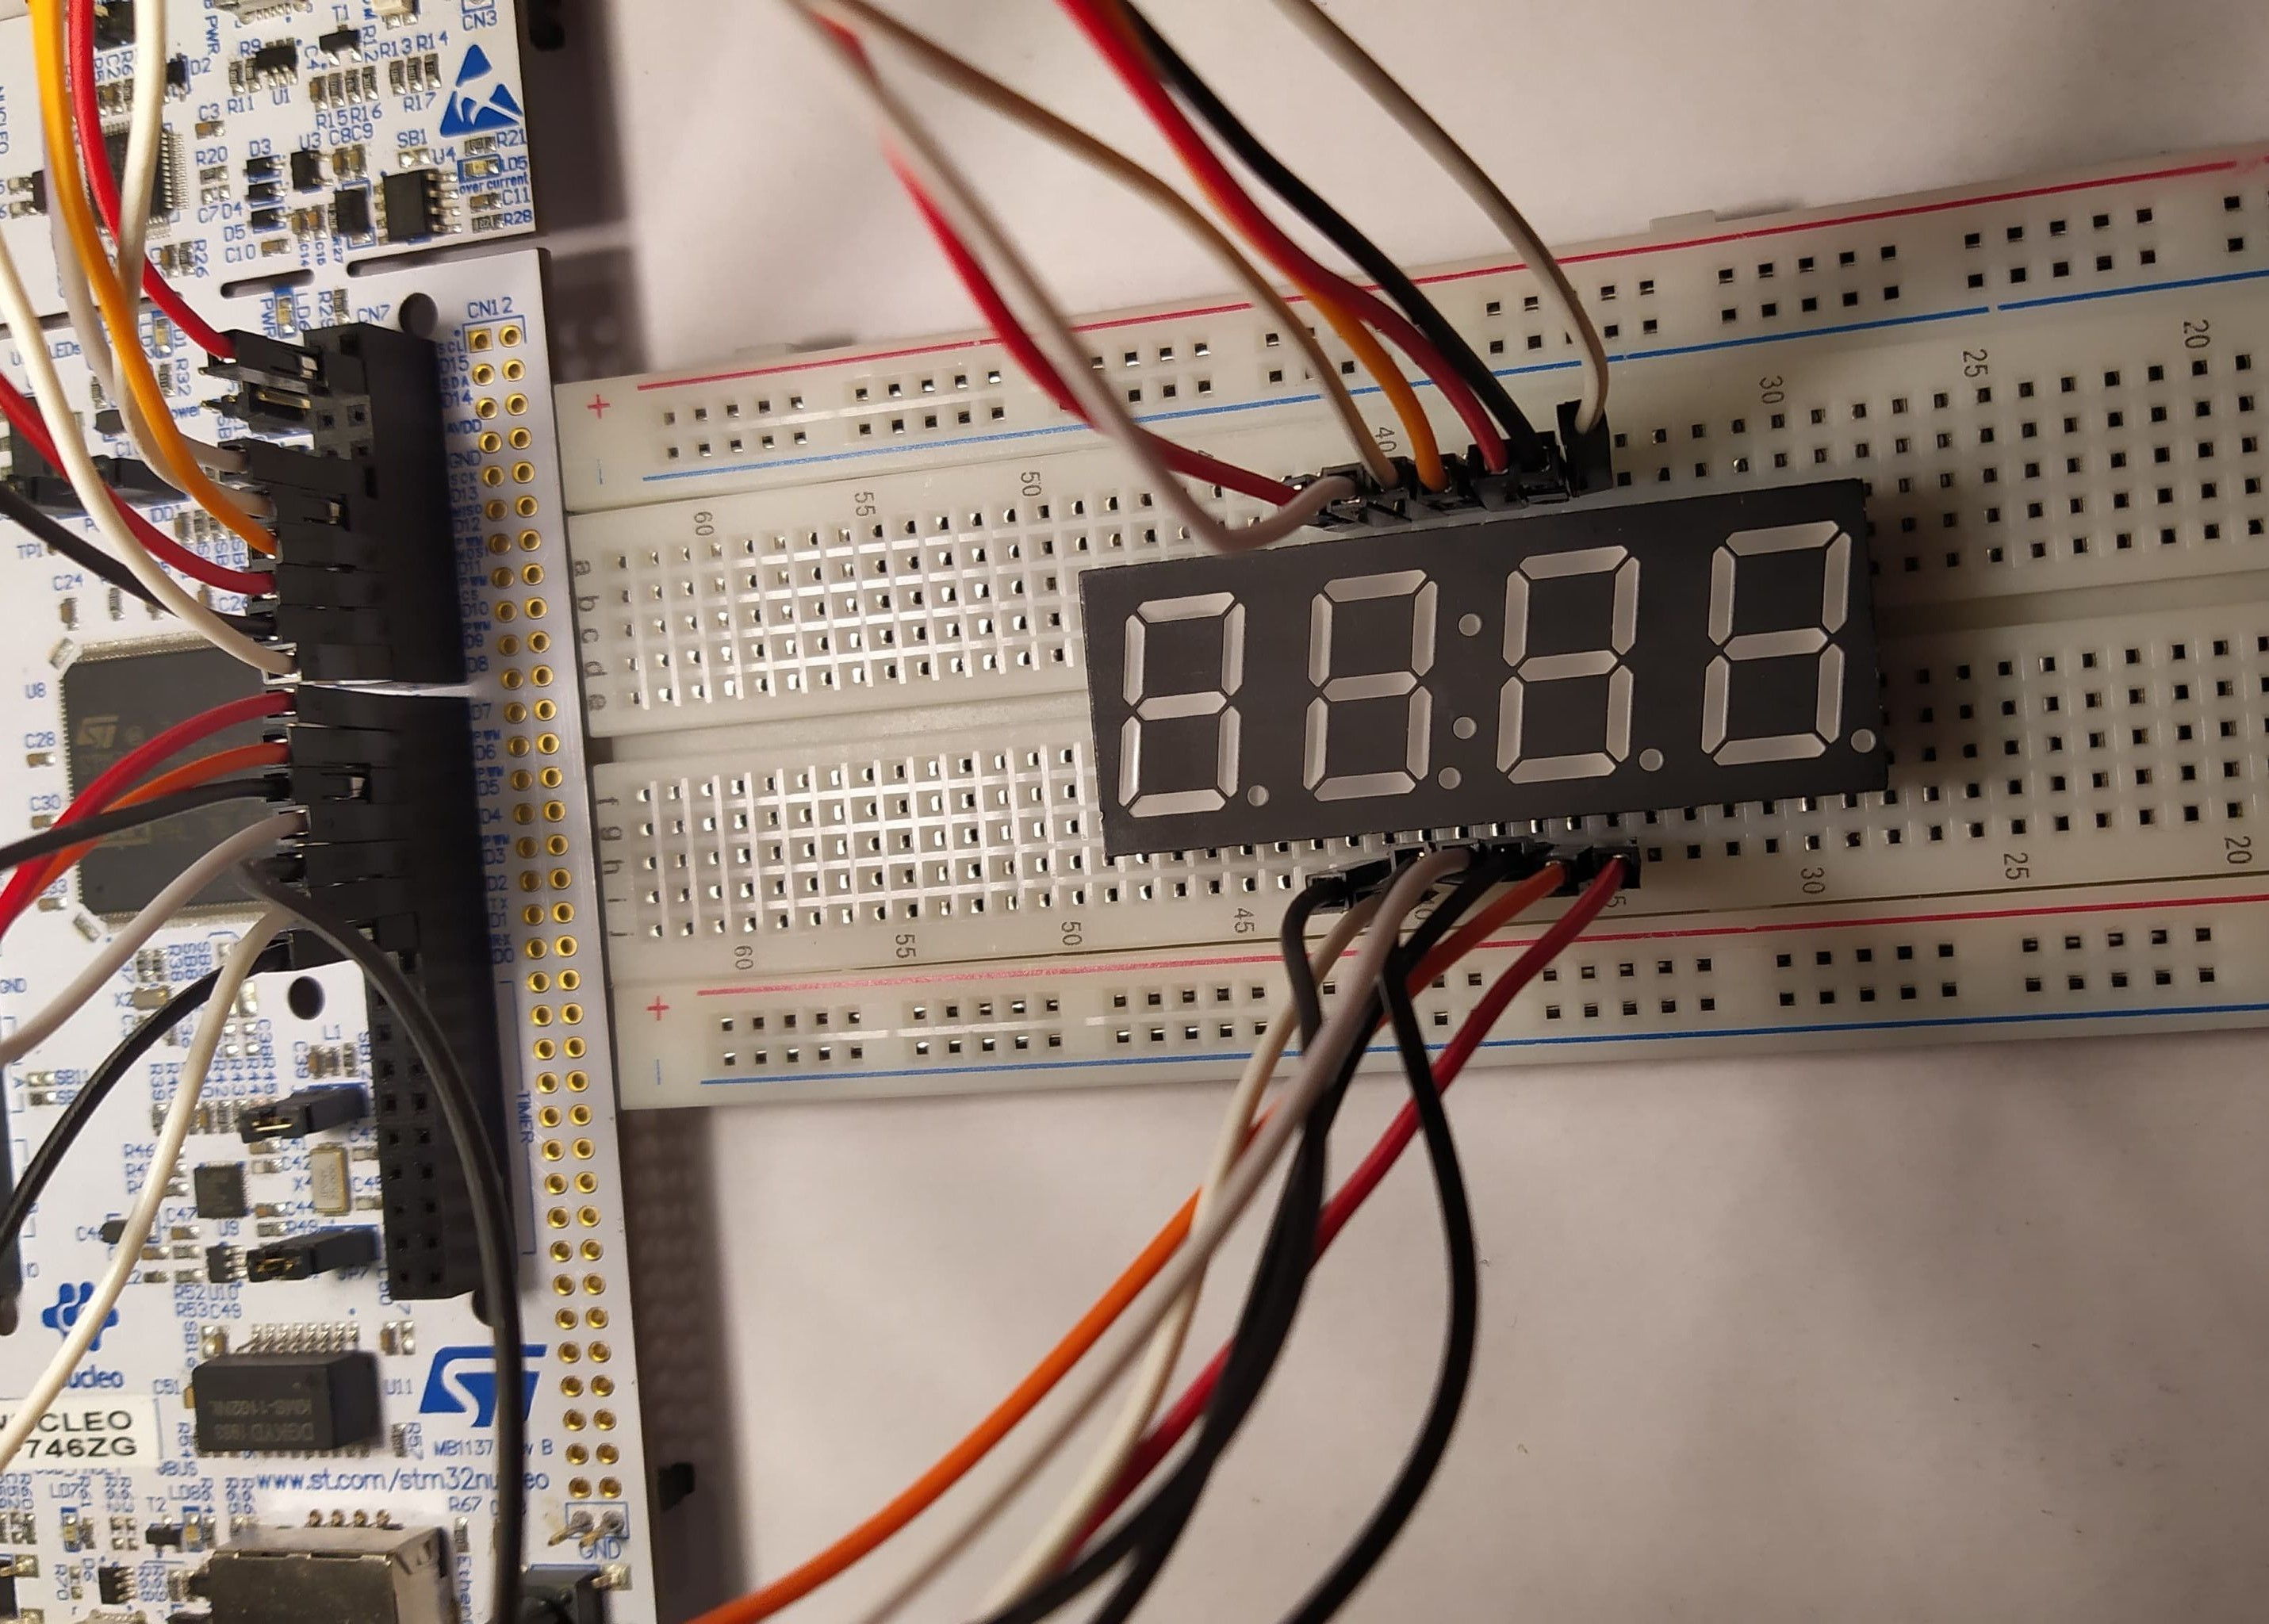
\includegraphics[width=0.6\textwidth]{fig/7Segment4DigitDisplay/zasada_dzialania/stm32Connection.jpg}
    \caption{Podłączenie układu pod mikrokontroler}
\end{figure}
A sam efekt końcowy programu otworzonego według powyżej określonych zasad wyglądał następująco:
\begin{figure}[H]
    \centering
    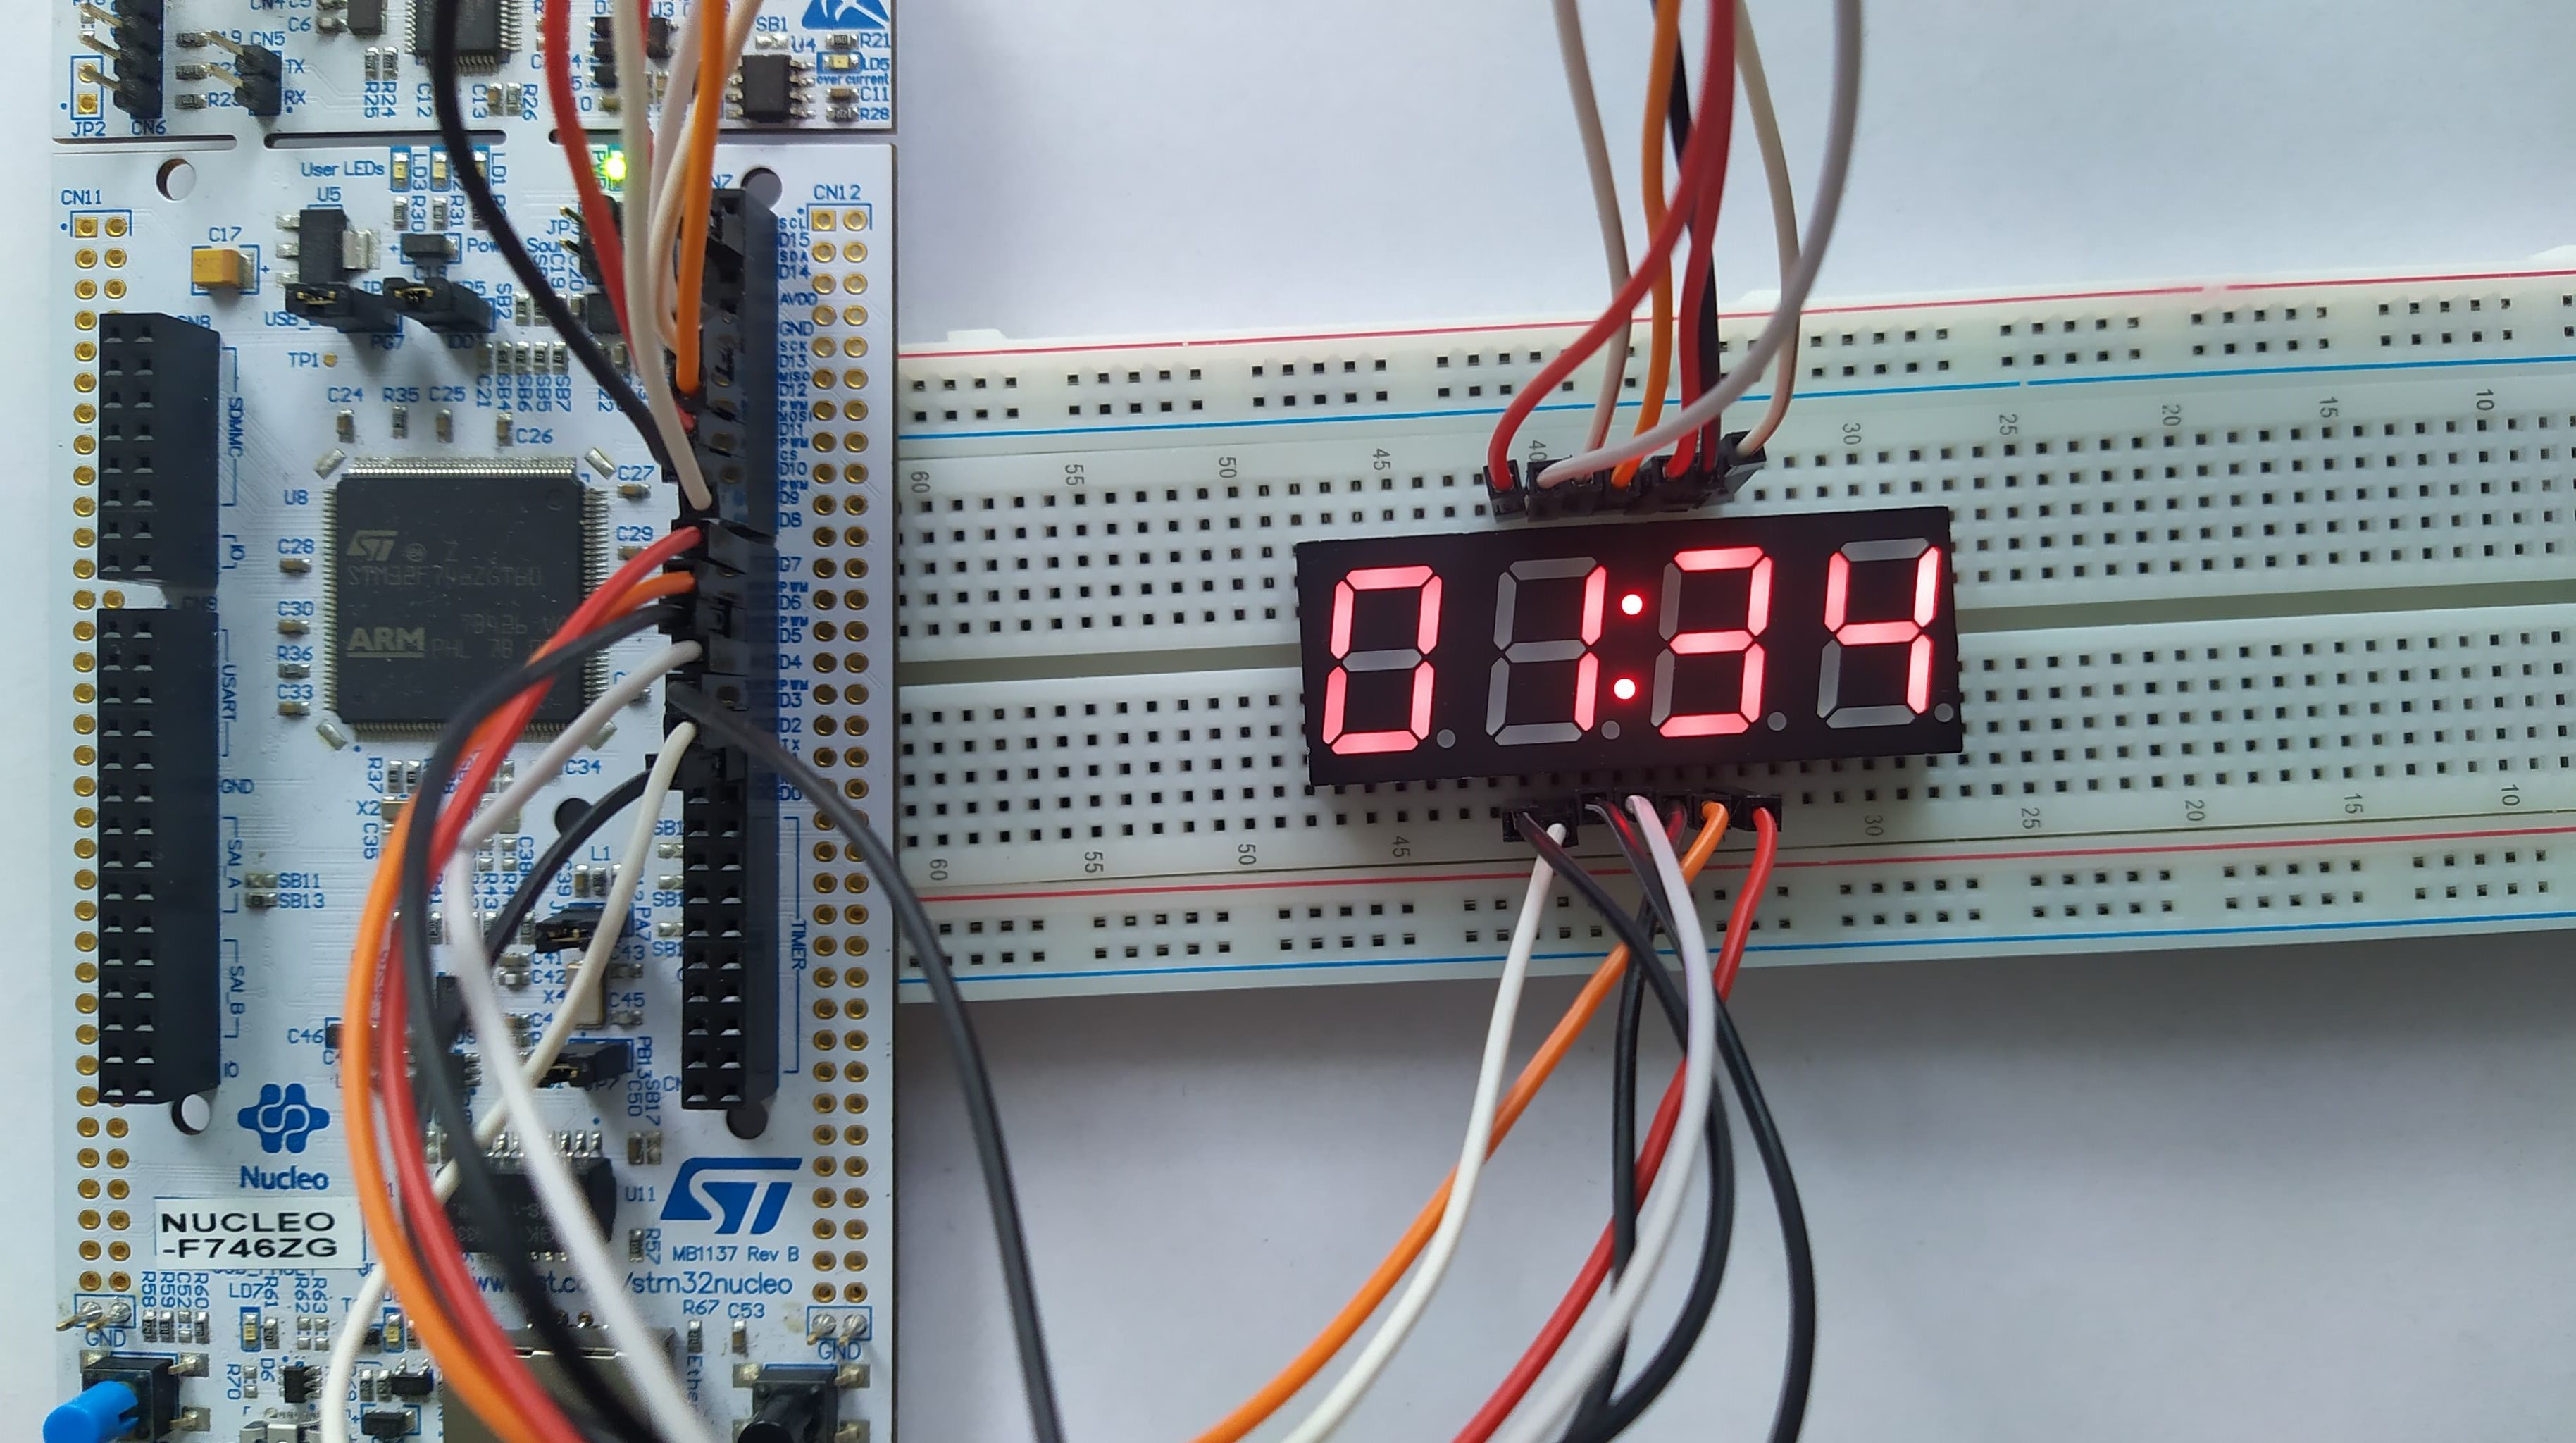
\includegraphics[width=0.6\textwidth]{fig/7Segment4DigitDisplay/zasada_dzialania/displayingDigits.jpg}
    \caption{Podłączenie układu pod mikrokontroler}
\end{figure}
Program co sekundę iterował wartość pojawiającą się następująco na wyświetlaczu. Konfiguracja pinów dla wyświetlacza musiała posiadać również odpowiednią konfigurację pinów GPIO\_Output, które posiadały następujące parametry:
\begin{itemize}
    \item Output Level - High(Wyświetlacz kompatybilny z pracą na 5V)
    \item GPIO mode - Output Push Pull
    \item Pull-up/Pull-down - Pull-down
    \item Maximum output speed - Very High
\end{itemize}

\newpage
\printbibliography[heading=bibintoc]

\end{document}